\documentclass{article}
\usepackage{fancyhdr}
\usepackage{titlesec}
\usepackage{graphicx}
\graphicspath{ {./img/} }
\usepackage{multirow}

\pagestyle{fancy}
\fancyhf{}
\lhead{Modul 7 Praktikum Jaringan Komputer}
\rfoot{\footnotesize Page \thepage}
\lfoot{\footnotesize Mahyus Ihsan, S.Si, M.Si \newline Jurusan Informatika Universitas Syiah Kuala \newline Modul oleh : Diky Wahyudi, Furqan Al Ghifari, Rendika Rahmaturrizki}
\renewcommand{\headrulewidth}{1pt}
\renewcommand{\footrulewidth}{1pt}

\titleformat*{\section}{\small\bfseries}

\begin{document}
    \begin{center}
        \textbf{Modul 7 Praktikum Jaringan Komputer}

        \textbf{Transport Layer dan Aplication Layer}
    \end{center}

    \section*{Deskripsi Singkat}

    \begin{flushleft}
        \textbf{Transport layer} merupakan sebuah lapisan transportasi. 
        Transport layer ini dapat menggabungkan beberapa koneksi transport ke dalam jaringan koneksi yang sama. 
        Transport Layer bertanggung jawab untuk menyampaikan data ke proses aplikasi yang sesuai pada komputer host.
        \newline

        \textbf{Application layer} merupakan layer ketujuh yang ada dalam Open Systems Interconnection (OSI) model dan menjadi satu-satunya layer yang dapat secara langsung berinteraksi dengan end user. 
        Layer ini terletak pada tingkat paling atas dan diizinkan oleh perangkat lunak atau user untuk mendapatkan akses ke jaringan. 
    \end{flushleft}

    \section*{Tujuan}
    \begin{enumerate}
        \item Dapat memahami konsep penggunaan port
        \item Dapat memahami berbagai macam protokol yang ada pada Aplication Layer
        \item Dapat melakukan konfigurasi DHCP Server, DNS Server dan Web Server
    \end{enumerate}

    \begin{flushleft}
        \textbf{Materi 1 - Port pada transport layer}
        \newline

        Port adalah mekanisme yang memungkinkan komputer terhubung dengan beberapa sesi koneksi dengan komputer dan program lainnya dalam jaringan.
        \newline

        Pada header protokol TPC/UDP yang telah dipelajari sebelumnya, terdapat bagian untuk \textbf{Source Port} dan \textbf{Destination Port}

        \begin{center}
            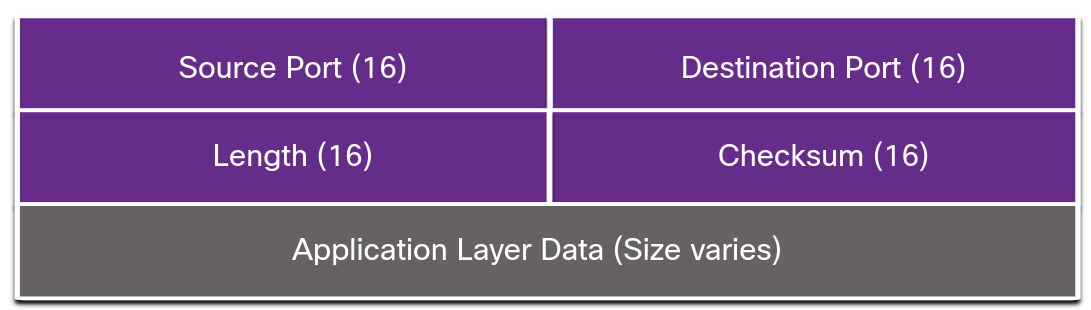
\includegraphics[scale=0.4]{1-2.png}
            Header UDP
        
            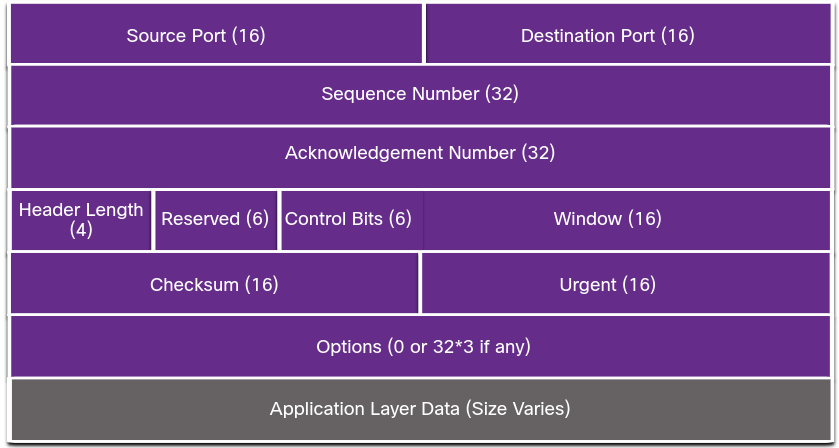
\includegraphics[scale=0.5]{1-1.png}
            Header TCP
        \end{center}

        Kelompok port :
        \begin{enumerate}
            \item \textbf{Well-Known Ports}
            Port ini memiliki angka dari 0 sampai 1,023. Port yang termasuk ke dalam well-known port, selalu merepresentasikan layanan jaringan yang sama, dan ditetapkan oleh Internet Assigned Number Authority (IANA).

            \item \textbf{Registered Ports}
            Port yang digunakan oleh vendor-vendor komputer atau jaringan yang berbeda untuk mendukung aplikasi dan sistem operasi yang mereka buat. 
            Registered port juga diketahui dan didaftarkan oleh IANA tetapi tidak dialokasikan secara permanen, sehingga vendor lainnya dapat menggunakan port number yang sama.

            \item \textbf{Private / Dynamic Ports}
            Port yang ditetapkan oleh sistem operasi atau aplikasi yang digunakan untuk melayani permintaan dari pengguna sesuai dengan kebutuhan.
        \end{enumerate}

        Contoh \textbf{Well-Known Ports} yang sering digunakan
        \begin{center}
            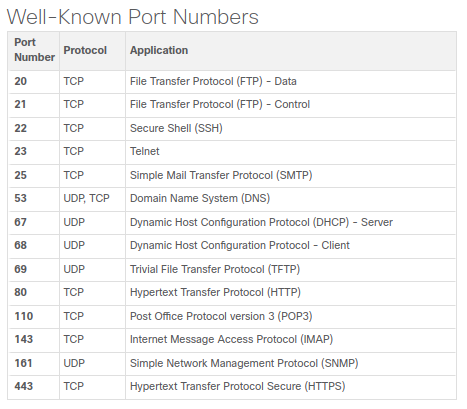
\includegraphics[scale=0.55]{1-3.png}
        \end{center}
    \end{flushleft}

    \begin{flushleft}
        \textbf{Materi 2 - Protokol pada Aplication Layer}
        \newline

        Beberapa protokol yang ada pada Aplication Layer :
        \begin{itemize}
            \item Name System
            \begin{enumerate}
                \item DNS - Domain Name System \newline
                Menterjemahkan domain menjadi IP address
            \end{enumerate}

            \item Host Config
            \begin{enumerate}
                \item BOOTP - Bootstrap Protocol \newline
                Protokol client-server yang dirancang untuk mendapatkan informasi yang diberikan di atas (yaitu, alamat IP, subnet mask, alamat router, alamat IP dari server nama)

                \item DHCP - Dynamic Host Configuration Protocol \newline
                Untuk memberikan IP pada Host secara dinamis
            \end{enumerate}

            \item Email
            \begin{enumerate}
                \item SMTP - Simple Mail Transfer Protocol \newline
                Berfungsi untuk mengirim dan menerima email antara server dan host

                \item POP3 - Post Office Protocol \newline
                Berfungi menerima email dan menyimpannya di dalam sebuah email server sampai ada user yang berhak mengakses akun tersebut

                \item IMAP - Internet Message Access Protocol \newline
                Berfungsi untuk mengakses email yang tersimpan pada server dan memanajemen email yang ada pada server
            \end{enumerate}

            \item File Transfer
            \begin{enumerate}
                \item FTP - File Transfer Protocol \newline
                Bergunsi untuk mengirim dan merima file antara server dan host

                \item TFTP - Trivial File Transfer Protocol \newline
                TFTP merupakan sebuah protokol sederhana untuk transfer file antar komputer yang sama maupun berbeda jaringan. TFTP dirancang khusus dengan ukuran kecil dan didimplementasikan
            \end{enumerate}

            \item Web
            \begin{enumerate}
                \item HTTP - Hypertext Transfer Protocol \newline
                Berfungi untuk membantu proses pertukaran data dalam internet antar komputer satu dengan lainnya

                \item HTTPS - HTTP Secure \newline
                Berfungsi untuk mengamankan komunikasi HTTP
            \end{enumerate}
        \end{itemize}
    \end{flushleft}

    \newpage
    \begin{flushleft}
        \textbf{Materi 3 - Konfigurasi DHCP Server, DNS Server dan Web Server}
        \newline

        \begin{enumerate}
            \item Buatlah jaringan seperti gambar berikut

            \begin{center}
                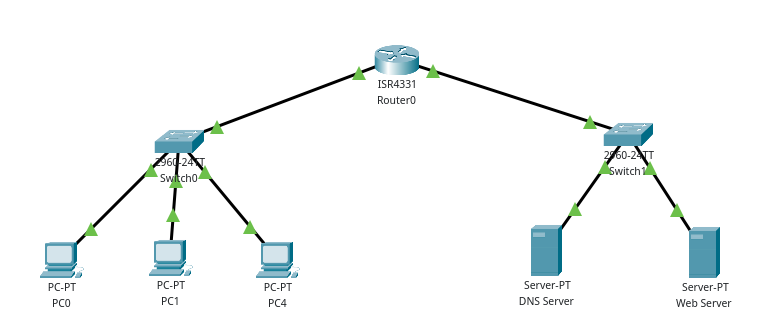
\includegraphics[scale=0.5]{3-1.png}
            \end{center}

            \item Kemudian berikan IP pada masing-masing switch, berdasarkan tabel berikut. Tetapi jangan lakukan konfigurasi pada PC terlebih dahulu

            \begin{tabular}{|c|c|c|c|c|}
                \hline
                Device & IP & Dest & Network & Gateway \\
                \hline
                \multirow{2}{4em}{Router0} & 192.168.1.1 & Switch0 & 192.168.1.0/29 & - \\
                & 192.168.1.9 & Switch1 & 192.168.1.8/29 & - \\
                \hline
                DNS Server & 192.168.1.10 & - & 192.168.1.8/29 & 192.168.1.9\\
                \hline
                Web Server & 192.168.1.11 & - & 192.168.1.8/29 & 192.168.1.9\\
                \hline
            \end{tabular}
            
            \begin{center}
                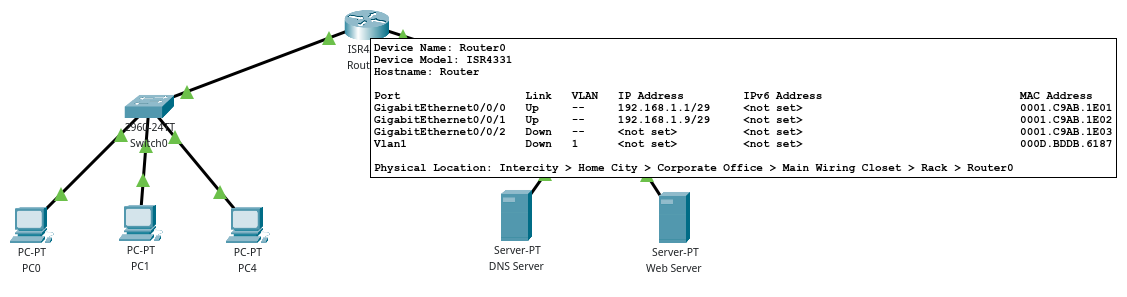
\includegraphics[scale=0.3]{3-2.png}
            \end{center}

            \item Kita akan melakukan konfigurasi DHCP pada network 192.168.1.0 pada router. Buka CLI pada router dan masuk ke dalam mode konfigurasi, dan lakukan konfigurasi seperti berikut.

            \begin{center}
                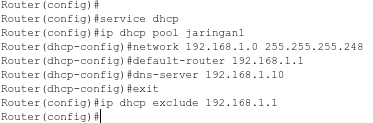
\includegraphics[]{3-3.png}
            \end{center}

            \item Setelah melakukan konfigurasi dhcp , pada PC masuk ke menu Desktop $>$ IP Configuration, kemudian pilih pilihan DHCP.
            
            \begin{center}
                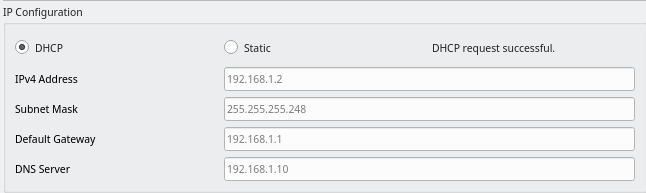
\includegraphics[scale=0.6]{3-4.png}
            \end{center}
            Maka IP akan diberikan secara otomatis. 
            Kemudian lanjutkan pada semua PC yang ada.

            \item Selanjutnya berikan IP pada Web Server secara static, sesuai dengan tabel diatas.

            \begin{center}
                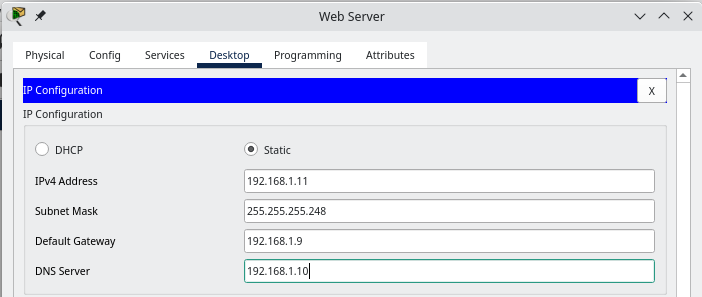
\includegraphics[scale=0.6]{3-5.png}
            \end{center}

            \item Pada web server aktifkan service HTTP dan HTTPS.
            
            \begin{center}
                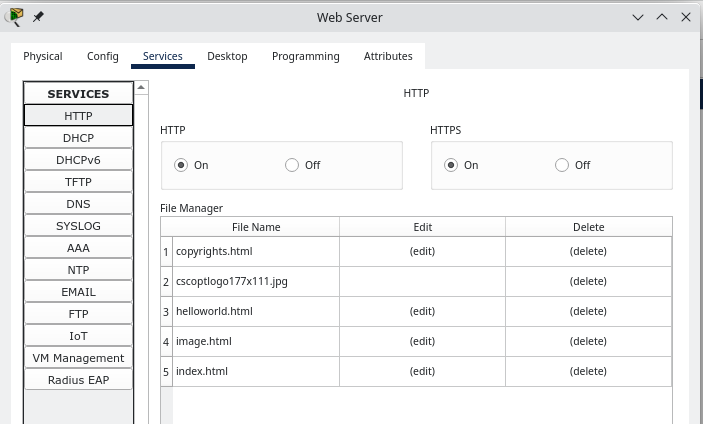
\includegraphics[scale=0.5]{3-6.png}
            \end{center}

            \item Pada PC buka Desktop $>$ Web Browser dan kemudian masukkan IP dari Web server pada kolom URL.
            
            \begin{center}
                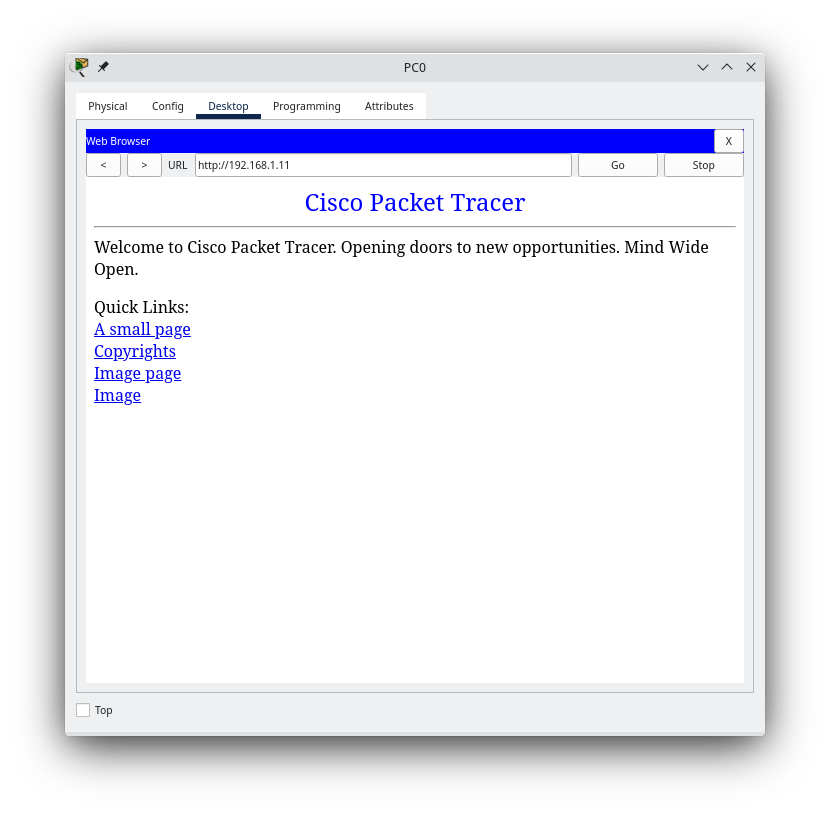
\includegraphics[scale=0.5]{3-7.png}
            \end{center}

            \item Karena kita tidak mungkin untuk menghafal semua IP dari web server yang kita gunakan maka dibuatlah DNS agar user lebih mudah dalam berkomunikasi. Lakukan konfigurasi IP pada DNS Server secara Statis.
            
            \begin{center}
                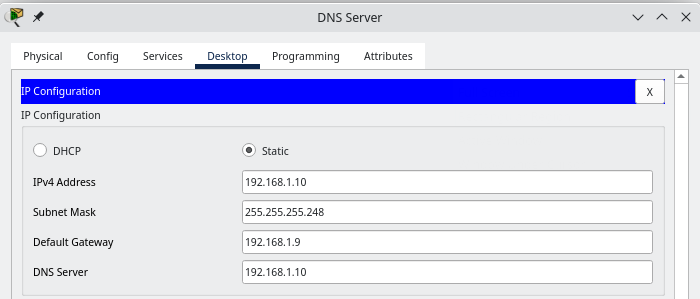
\includegraphics[scale=0.6]{3-8.png}
            \end{center}

            \item Hidupkan Service DNS pada DNS Server
            
            \begin{center}
                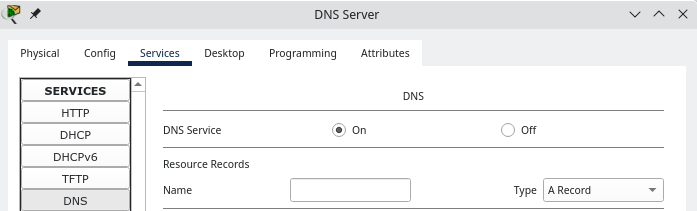
\includegraphics[scale=0.6]{3-9.png}
            \end{center}

            \item Tambahkan nama domain dan address pada DNS, nama domain terserah (ex. terserah.com) dan masukkan address dari Web Server yang telah kita buat tadi. Kemudian tekan tombol \textbf{Add}
            
            \begin{center}
                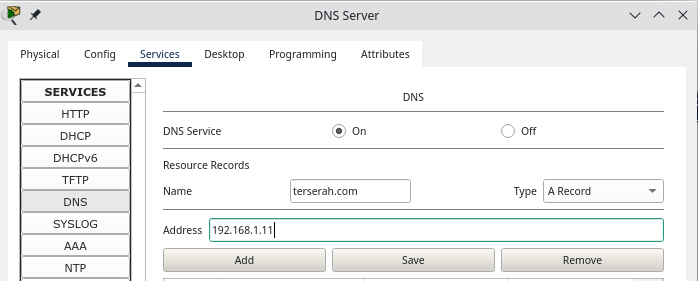
\includegraphics[scale=0.6]{3-10.png}
            \end{center}

            \item Sekali lagi pada PC buka Desktop $>$ Web Browser dan kemudian masukkan nama domain yang kita isikan pada DNS Server tadi.
            
            \begin{center}
                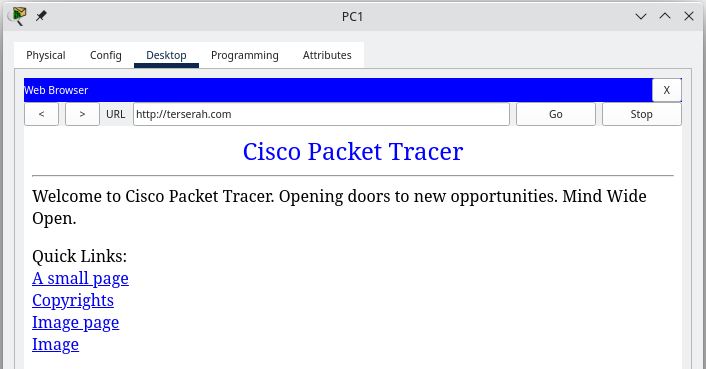
\includegraphics[scale=0.5]{3-11.png}
            \end{center}

            \item Maka domain sudah terdaftar pada DNS dan tidak perlu lagi untuk menuliskan IP setiap kali akan berkomunikasi dengan device lain.

            \item DNS tidak terbatas hanya kepada server, semua ip yang ada pada jaringan bisa dimasukkan ke dalam DNS.

            \item Buatlah sebuah PC baru dengan nama PC Admin dan berikan IP 192.168.1.12
            \begin{center}
                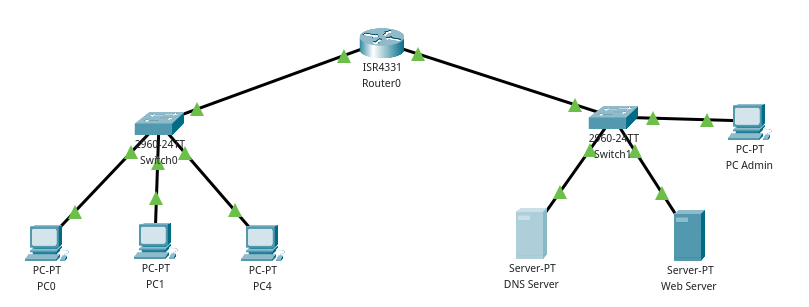
\includegraphics[scale=0.5]{3-12.png}
            \end{center}

            \item Pada DNS Server tambahkan IP PC Admin.
            \begin{center}
                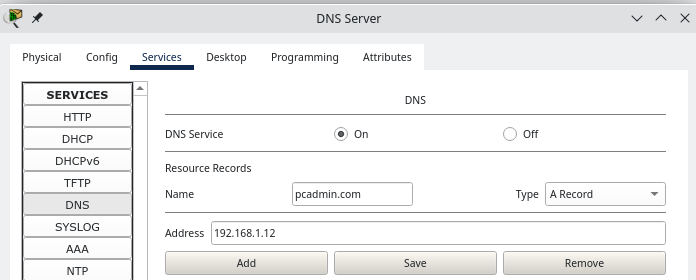
\includegraphics[scale=0.5]{3-13.png}
            \end{center}

            \item Sekarang untuk berkomunikasi dengan PC Admin tidak perlu untuk memasukkan IP lagi , tinggal memasukkan domain dari PC Admin yang telah ditambahkan ke DNS Server.
            \begin{center}
                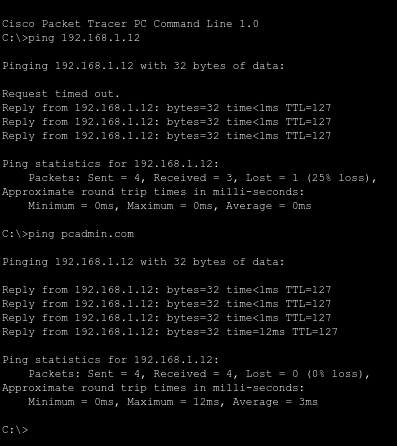
\includegraphics[scale=0.5]{3-14.png}
            \end{center}
        \end{enumerate}
    \end{flushleft}
\end{document}
